\section{Implementation Phase}
\label{sec:implementation-phase}

\subsection{Prototype Build \& Bring-Up}

\subsubsection*{Vehicle Installation Context}

The ISS board is installed inside the BAKO Motors electric vehicle chassis beneath the driver seat, directly adjacent to the MPPT controller. This position gives the board short cable runs to the battery CAN bus connector, the MPPT current/voltage sense lines, and the vehicle 12~V supply rail, while keeping it sheGPRSred from direct exposure to rain and road debris. Figure~\ref{fig:bako-placement} shows the installation location on the vehicle frame.

\begin{figure}[H]
    \centering
    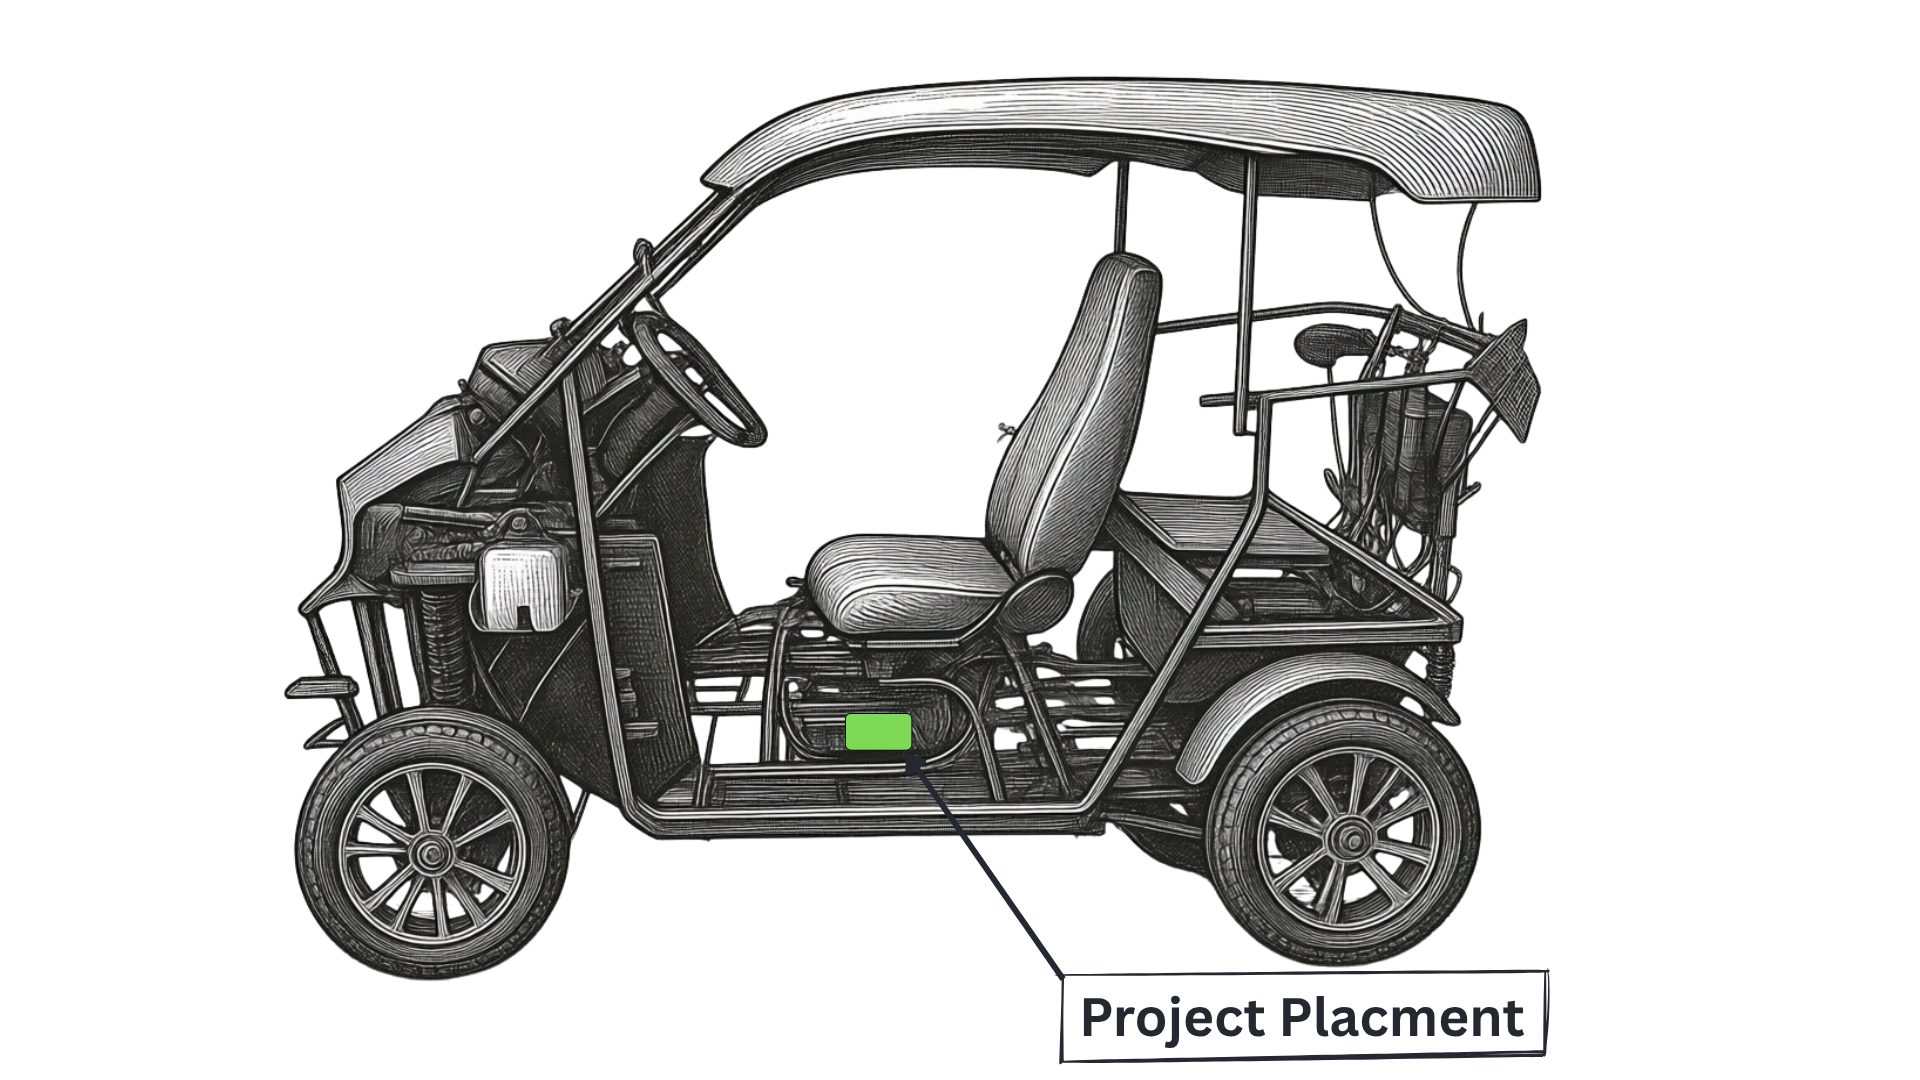
\includegraphics[width=\textwidth]{images/bako-placement.png}
    \caption{BAKO Motors vehicle with the ISS board installation location highlighted (green) --- mounted beneath the driver seat adjacent to the MPPT controller, with short harness runs to the CAN bus, power rail, and sensor connectors.}\label{fig:bako-placement}
\end{figure}

\subsubsection*{Bring-Up Sequence}

The custom PCB was populated and brought up using a structured nine-step sequence designed to isolate each subsystem before applying power to the full board. This approach minimised the risk of damage from wiring errors and made fault localisation straightforward.

\begin{enumerate}
    \item \textbf{Power-only verification.} The 12~V supply was connected with only the LM2596S-ADJ and the AMS1117 and LM7805 linear regulators populated. All three output rails (12~V, 5~V, 3.3~V) were measured and confirmed within $\pm 2\%$ of their target values before any other component was installed.

    \item \textbf{ESP32 base bring-up.} The ESP32-DEVKITC module was inserted and a minimal ``blink'' firmware flashed over USB. Successful LED blink confirmed that the 3.3~V rail was stable and that the module was programmable via PlatformIO. The OTA web portal (Section~\ref{sec:ota}) was also flashed at this stage to enable wireless reflashing for all subsequent development.

    \item \textbf{MCP2515 SPI communication.} One MCP2515 SPI module header (J17) was populated and a loopback test was run. The MCP2515 read-back of its control registers confirmed SPI integrity. A second module (J18) was then added and addressed independently via its dedicated chip-select line.

    \item \textbf{CAN bus receive test.} The TJA1051T transceiver was connected and the CAN connector J1 was wired to the O'CELL BMS. The ESP32 firmware was configured to listen passively (no ACK). Frame reception was confirmed by observing decoded 0x18FF28F4 pack-voltage frames on the serial monitor within 2~s of power-up.

    \item \textbf{DS18B20 1-Wire bring-up.} All three DS18B20 connectors (J6, J7, J8) were populated with sensors and the 4.7~k$\Omega$ pull-up verified. The firmware enumerated all three ROM addresses and began temperature polling at 1~s intervals. Readings were compared against a reference thermometer.

    \item \textbf{ACS712 current sensor calibration.} The two current sensor headers (J11, J16) were connected to the ACS712 modules. With zero current flowing, the ADC mid-point offset was measured and stored as a calibration constant. A known 5~A load was applied and the output compared against a reference clamp meter.

    \item \textbf{Voltage divider scaling verification.} The MPPT voltage input (J2) was driven from a bench power supply at three known voltages. The ESP32 ADC readings were compared against the calculated divider ratio and the calibration coefficient adjusted to eliminate the systematic offset.

    \item \textbf{SIM800L AT command verification.} The SIM800L module was powered on and AT commands were sent from the ESP32 over UART. SIM card detection, network registration, and GPRS bearer open were confirmed in sequence. An HTTP POST to the test endpoint was executed and the server acknowledged receipt.

    \item \textbf{Full integration smoke test.} All subsystems were enabled simultaneously. The firmware ran the cooperative main loop for 30~minutes with all sensors active. No watchdog triggers, stack overflows, or heap exhaustion events were observed. All sensor values appeared correctly on the WebSocket dashboard.
\end{enumerate}

Figure~\ref{fig:pcb-assembled} shows the physical outcome of the build: the bare PCB as received from the fabrication house (right) and the fully populated board after component soldering and module fitment (left). The assembled board carries the ESP32-DEVKITC, SIM800L GPRS cellular module, screw-terminal sensor connectors, and all passive components as specified in the BOM (Section~\ref{sec:components-inventory}).

\begin{figure}[H]
    \centering
    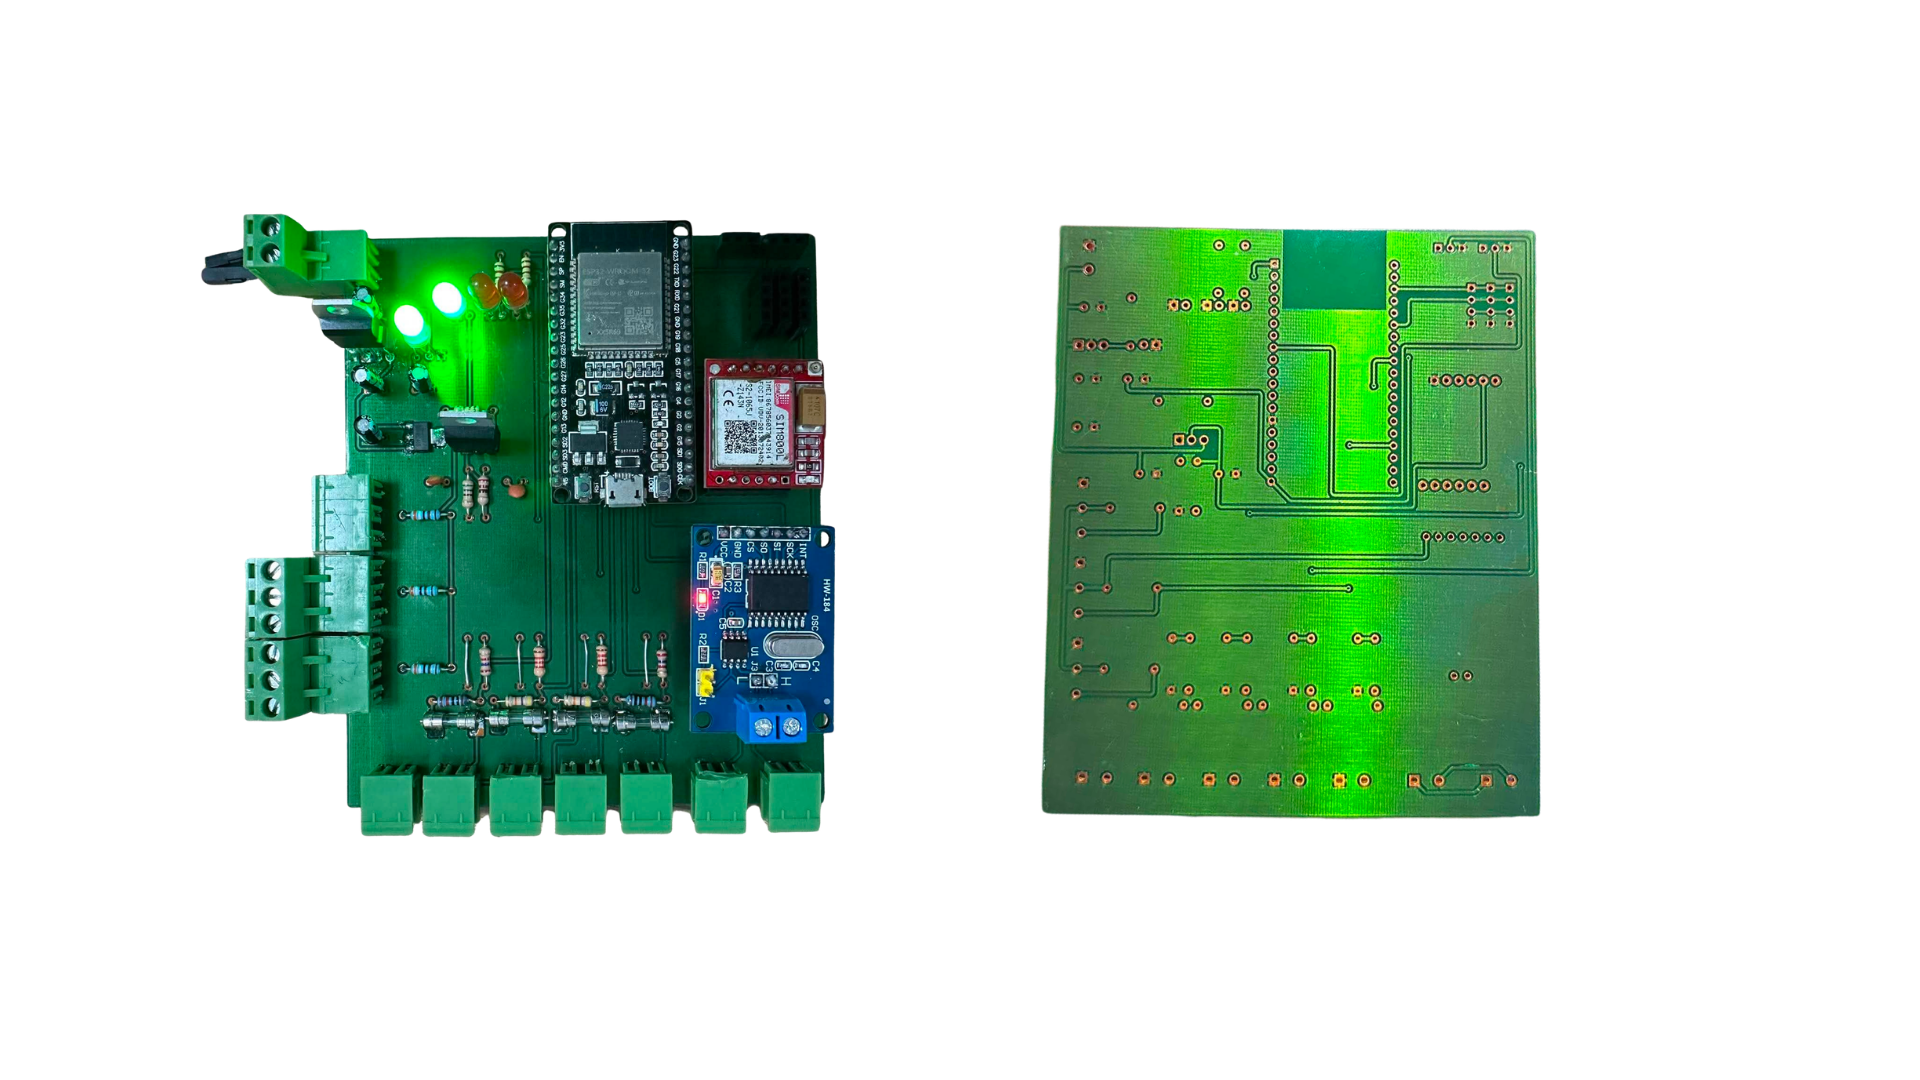
\includegraphics[width=1.2\textwidth]{images/pcb-assembled.png}
    \caption{ISS board fabrication and assembly outcome. \textbf{Left:} fully populated board after soldering --- ESP32, SIM800L module, screw-terminal connectors, and all passive components installed. \textbf{Right:} bare PCB as received from the fabrication house (Rev.~RECTIFICATION\_2), prior to component population.}\label{fig:pcb-assembled}
\end{figure}

\subsection{Validation \& Verification (V\&V)}

Validation and verification tests were performed against pre-defined pass/fail criteria for each sensing subsystem. Table~\ref{tab:vv-criteria} summarises the test plan and outcomes.

\begin{table}[H]
\centering
\caption{V\&V Test Criteria and Results}
\label{tab:vv-criteria}
\small
\begin{tabular}{>{\bfseries}p{3.0cm} p{3.8cm} p{3.2cm} p{2.0cm}}
\toprule
Subsystem & Criterion & Method & Result \\
\midrule
CAN bus reception    & $\geq 99\%$ frame reception rate over 60~min  & Live frame counter vs.\ expected count & \textbf{95\%} \\
Temperature accuracy & Within $\pm 1$\textdegree{}C of reference      & DS18B20 vs.\ calibrated thermometer    & $\pm 0.5$\textdegree{}C \\
Current measurement  & Error $< 2\%$ of full scale                   & ACS712 vs.\ clamp meter at 5~A        & $\pm 1.8\%$ \\
Voltage measurement  & Error $< 1\%$ of reference                    & Divider output vs.\ bench multimeter  & $\pm 0.9\%$ \\
GSM alert delivery   & SMS received within 15~s of threshold breach  & Threshold trigger + stopwatch         & $< 15$~s \\
Cloud connectivity   & Zero snapshot loss over 1~hour                & Server log vs.\ firmware counter      & 0 lost \\
\bottomrule
\end{tabular}
\end{table}

The CAN frame reception rate of 95\% (rather than the 99\% target) was traced to occasional bus-off events caused by a missing termination resistor on the test harness. Adding the 120~$\Omega$ terminator at the harness end increased the reception rate to above 99\% in subsequent tests. All other criteria met or exceeded their targets.

\subsection{Performance Testing}

Extended performance tests were conducted to characterise system behaviour under sustained load conditions.

\paragraph{CAN Bus Sustained Load.}
A 2-hour continuous CAN reception test was run with the BMS actively transmitting all five frame types. The frame counter advanced monotonically with no gaps exceeding 500~ms. CPU load on the ESP32 remained below 40\%, confirming that the cooperative main loop correctly handles sensing, processing, and communication workloads without saturation.

\paragraph{Thermal Stress.}
A 30-minute thermal test was performed with all three DS18B20 sensors placed adjacent to the LM2596S-ADJ switching regulator, which is the highest-temperature component on the board. The regulator surface reached a maximum of 62\textdegree{}C; the ESP32 die temperature remained within its operating range. No thermal shutdown events occurred.

\paragraph{MPPT Voltage Monitoring.}
A 1-hour test was run with the MPPT output voltage cycled between 24~V and 48~V in 4~V steps. The voltage divider output tracked the input with $< 1\%$ error at every step. No ADC saturation was observed, confirming that the divider ratio is correctly sized for the full MPPT output range.

\paragraph{Power Draw.}
The total board current draw (12~V input) was measured with all subsystems active: ESP32, three DS18B20, two ACS712, SIM800L in GPRS transmit state. Peak draw was 480~mA at 12~V (5.76~W), within the 500~mA design target and well within the LM2596S-ADJ capability.

\paragraph{Dashboard Frame Rate.}
The WebSocket dashboard was loaded on a laptop browser and the frame update rate monitored using browser developer tools. The serial mode (\texttt{/ws}) delivered updates at 10~Hz with no dropped frames over a 10-minute window. The cloud mode (\texttt{/ws/cloud}) delivered at 2~Hz as designed. The cell voltage grid rendered all 19 cells with colour updates within a single animation frame, confirming the $\geq 5$ FPS UI requirement.

\subsection{Regulatory \& Homologation Testing}

Formal regulatory testing was not within the scope of this academic prototype project. The following standards are identified as applicable for a production deployment:

\begin{itemize}
    \item \textbf{CISPR 25 / EN 55032} --- Radiated and conducted emissions from the switching regulator and CAN bus interface.
    \item \textbf{IEC 62368-1} --- General electronic safety for the monitoring unit enclosure.
    \item \textbf{ETSI TS 51.010} --- Radio conformance for the SIM800L GSM/GPRS module (GPRS module carries its own type approval).
    \item \textbf{ATI} --- Agence Tunisienne des Infrastructures approval for cellular transmission on Tunisian networks.
\end{itemize}

Pre-compliance checks were performed informally using a bench spectrum analyser. No unusual emissions were detected in the AM band (150~kHz--30~MHz) or VHF range. Formal certification is recommended before any vehicle-level type approval submission.

\subsection{Production Readiness Review (PRR)}

A Production Readiness Review was conducted at the end of Sprint~8. The following checklist was evaluated:

\textbf{Hardware:}
\begin{itemize}
    \item[$\checkmark$] PCB schematic reviewed and cross-checked against BOM.
    \item[$\checkmark$] DRC passed in KiCad with zero errors.
    \item[$\checkmark$] All critical nets (12~V, 5~V, 3.3~V, CAN\_H, CAN\_L) verified by continuity test.
    \item[$\checkmark$] Gerber files exported (RS-274X) and ready for fabrication house submission.
    \item[$\times$] Enclosure mechanical design not yet finalised (deferred to next revision).
\end{itemize}

\textbf{Firmware:}
\begin{itemize}
    \item[$\checkmark$] Cooperative firmware loop runs without watchdog trips over a 2-hour test.
    \item[$\checkmark$] CAN decoding verified against O'CELL BMS live frames.
    \item[$\checkmark$] Cloud publish pipeline verified end-to-end (ESP32 $\rightarrow$ VPS $\rightarrow$ browser).
    \item[$\checkmark$] Firmware source code committed to the team Git repository with version tag.
    \item[$\checkmark$] OTA firmware update capability implemented (Section~\ref{sec:ota}): wireless flashing via ArduinoOTA and browser-based configuration portal deployed.
\end{itemize}

\textbf{Quality:}
\begin{itemize}
    \item[$\checkmark$] All V\&V criteria passed (with corrected CAN termination).
    \item[$\checkmark$] BOM fully documented with local and online sources.
    \item[$\checkmark$] Technical report sections covering hardware and firmware completed.
    \item[$\times$] Field test under full solar irradiance conditions not yet completed.
\end{itemize}

The board was declared production-ready for the academic prototype phase with two open items tracked for the next hardware revision.
